\documentclass[border=10pt]{standalone}
\usepackage{pgfplots}
\pgfplotsset{compat=1.18}
\begin{document}
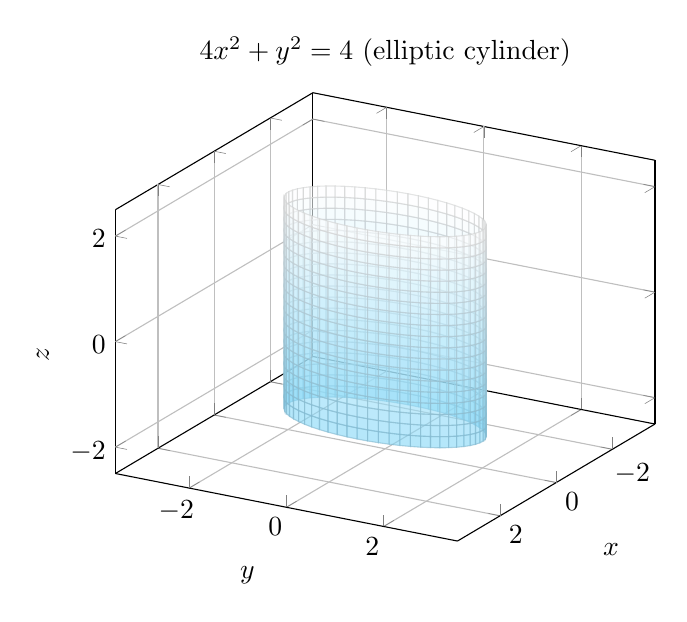
\begin{tikzpicture}
\begin{axis}[
    xlabel={$x$}, ylabel={$y$}, zlabel={$z$},
    xmin=-2, xmax=2, ymin=-2.5, ymax=2.5, zmin=-2.5, zmax=2.5,
    axis equal,
    view={120}{20},
    grid=major,
    title={$4x^2+y^2=4$ (elliptic cylinder)},
    samples=60, samples y=20
]
\addplot3[surf, domain=0:360, y domain=-2:2, z buffer=sort, opacity=0.6, colormap={bw}{color=(cyan!50) color=(white)}]
    ({cos(x)}, {2*sin(x)}, {y});
\end{axis}
\end{tikzpicture}
\end{document}
